
\section{Bus Système : Le PIBUS}

Le bus permettant d'interconnecter les processeurs avec les autres composants.
\begin{center}
  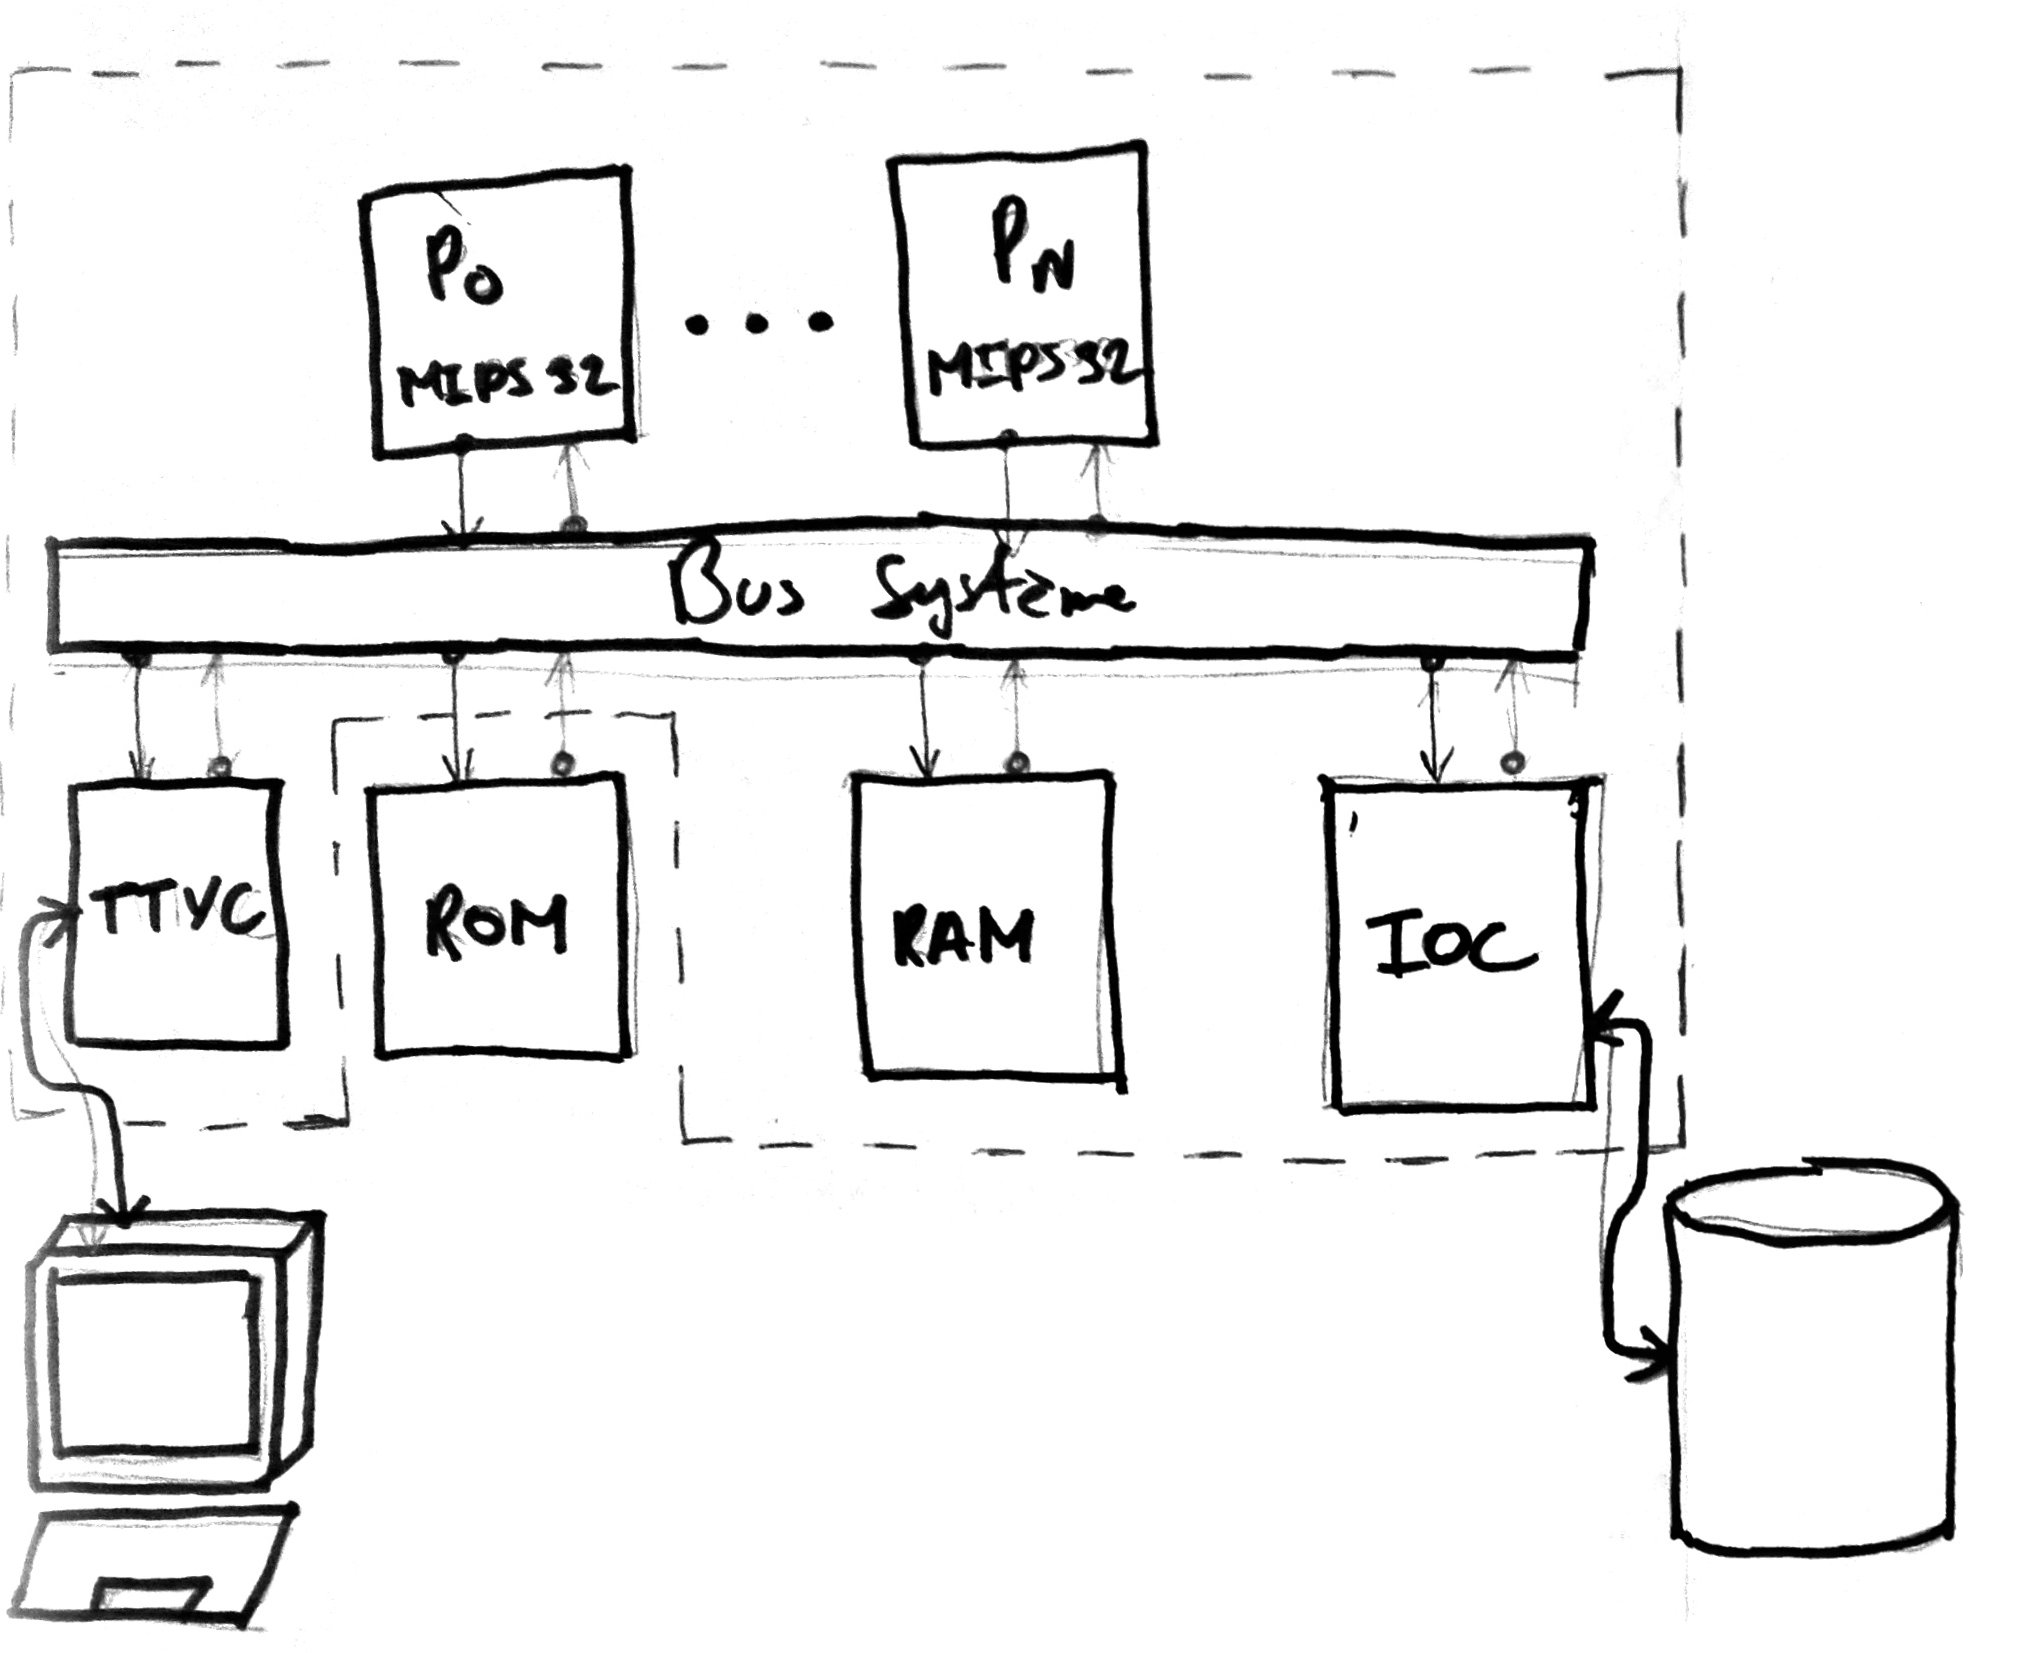
\includegraphics[height=11cm]{cours2/pics/bus.jpg}
\end{center}
De nos jours, le bus ne se contente plus d'être une simple nappe de fils, il s'agit d'un
réseau d'interconnection sur puce. Le bus est devenu un composant crucial des
machines.
\begin{center}
  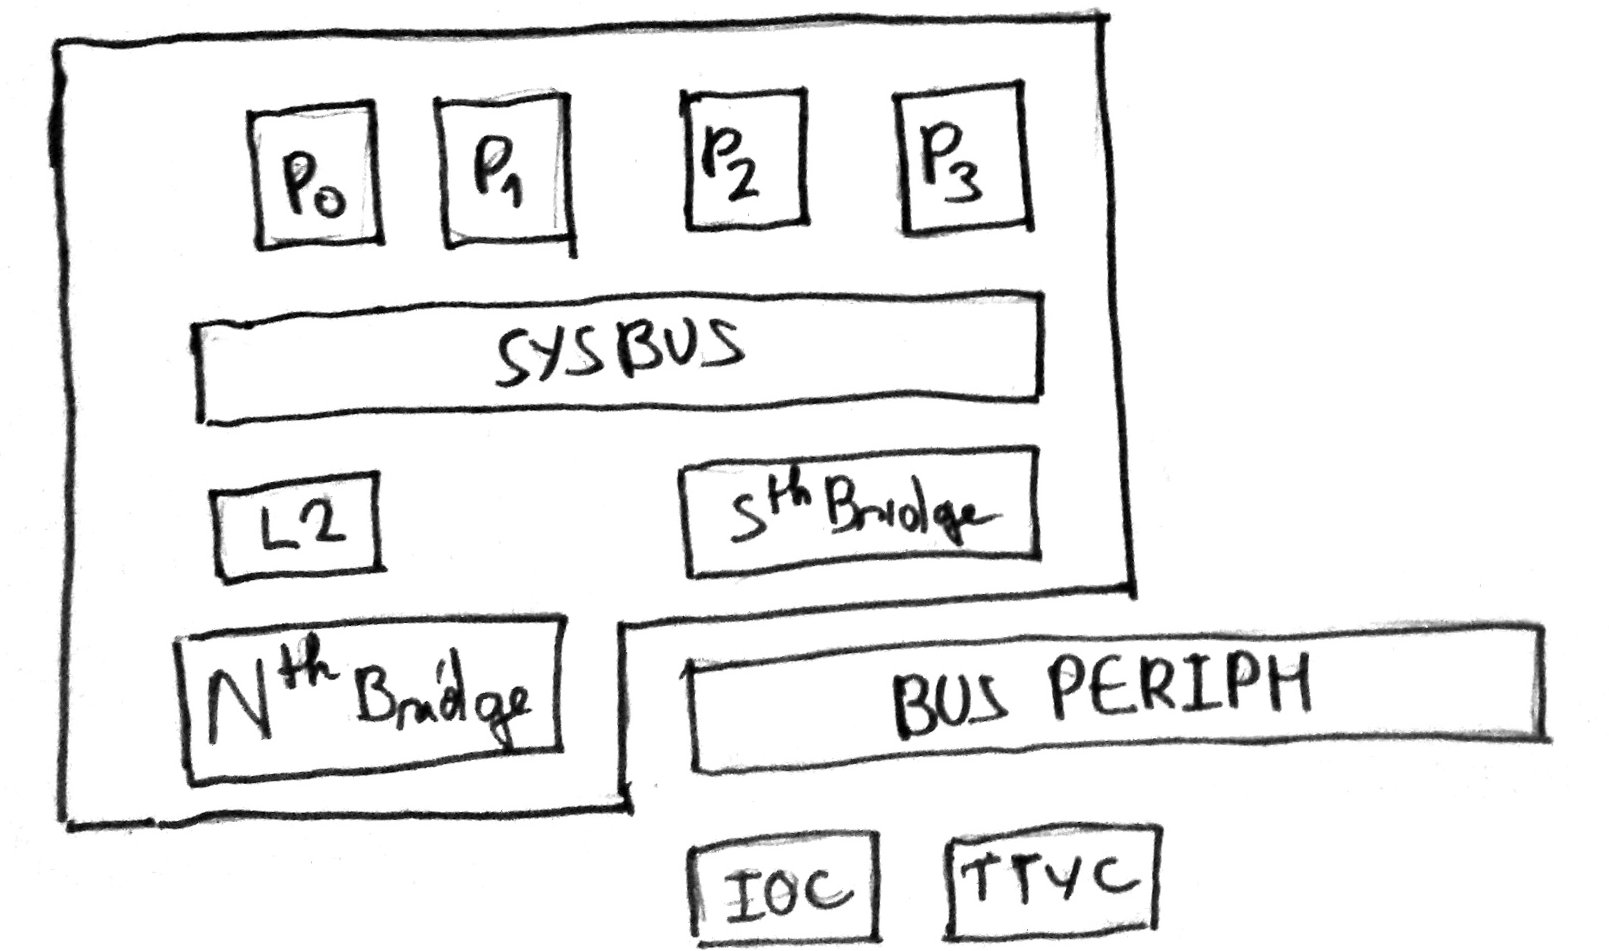
\includegraphics[height=5cm]{cours2/pics/modern.jpg}\\
  {\it Le North Bridge fait transiter les données vers la RAM, le South Bridge
  vers le bus périphérique. Tous deux sont des contrôleurs sur puce.}
\end{center}

\section{Fonctions d'un bus}
\begin{enumerate}
  \item Acheminemenr des commandes des maîtres vers les bonnes cibles :
  \begin{itemize}
    \item routage vers la bonne cible
    \item routage vers les différents maîtres
  \end{itemize}
  \item Acheminement des réponses des cibles vers le bon maître
  \begin{itemize}
    \item arbitrage entre les cibles
  \end{itemize}
\end{enumerate}\begin{center}
  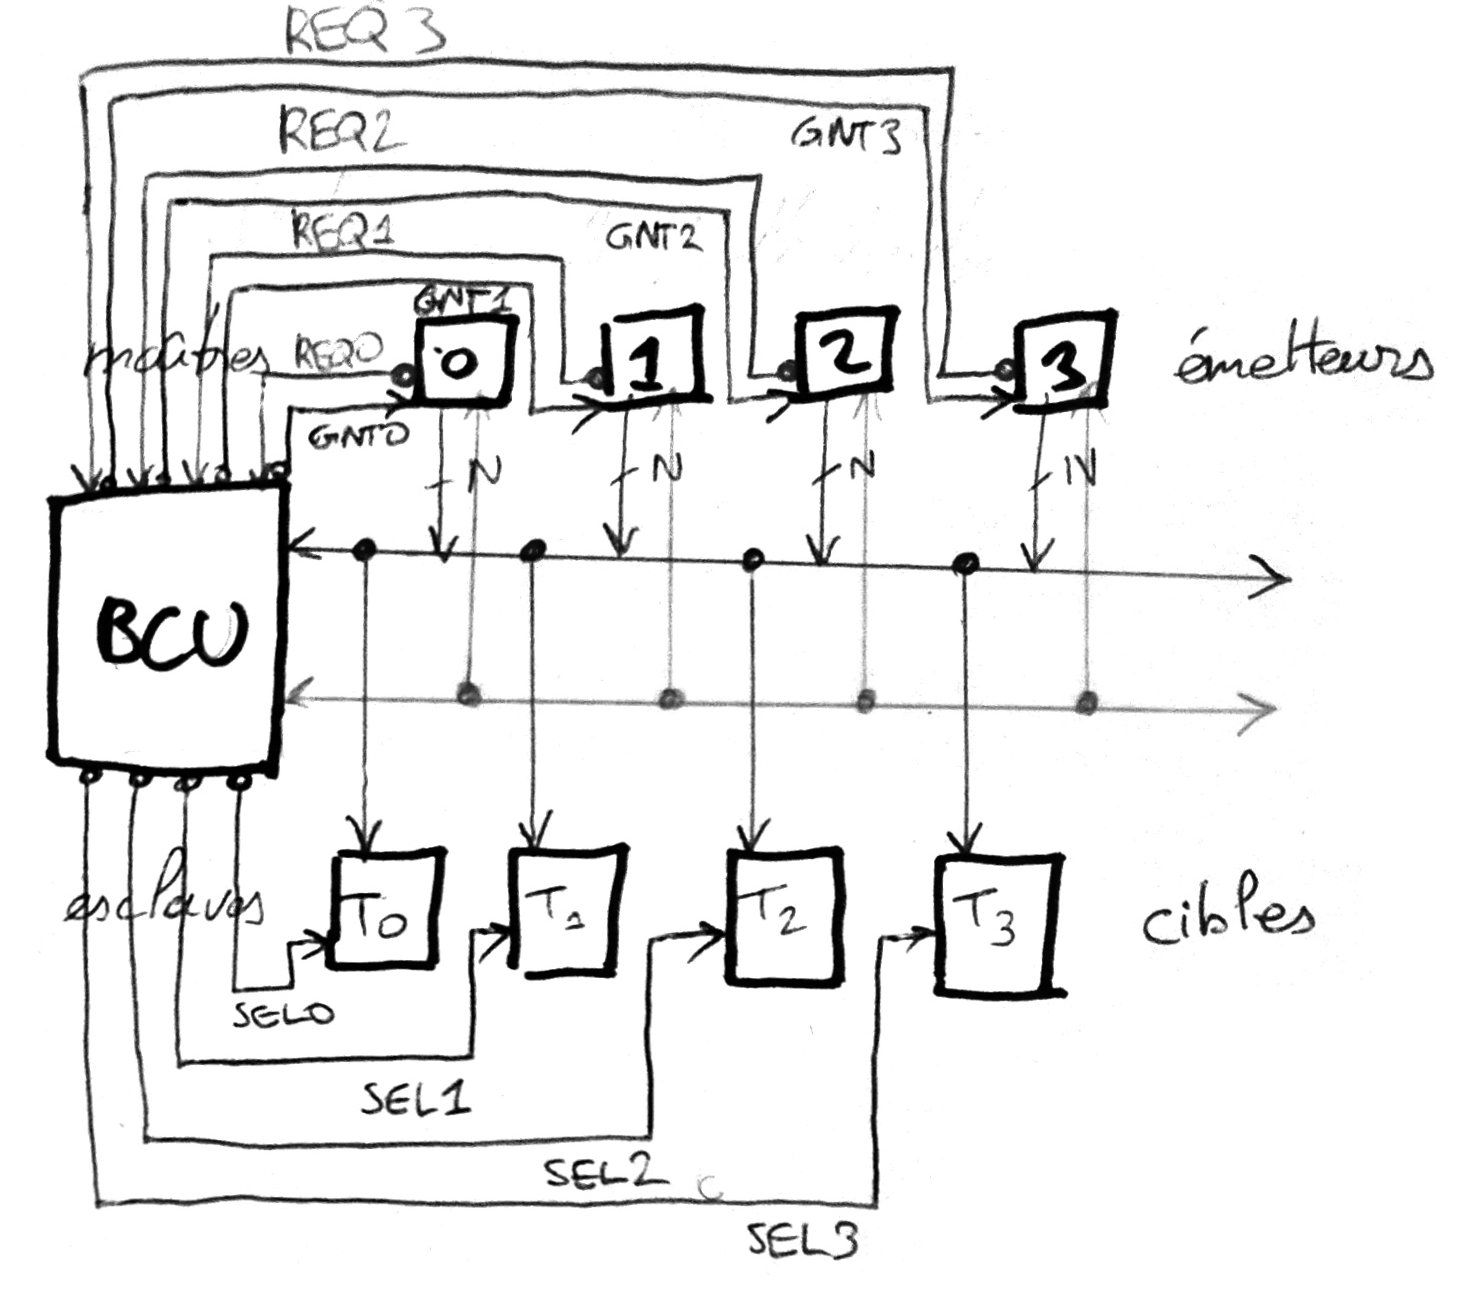
\includegraphics[height=11cm]{cours2/pics/bcu.jpg}
\end{center}
{\it\bf transaction} : paire d'une commande d'un maître et d'une réponse de la cible.\\
Cela est vrai pour les lectures {\bf et} les écritures, et ce afin de :
\begin{itemize}
  \item notifier d'éventuelles erreurs, et permettre un deboguage plus exhaustif.
  \item {\bf prévenir de problèmes de synchronisation}\\
  Exemple : \\
  Deux applications multithreadées communicantes par une case mémoire : système
  producteur/consommateur. Le producteur doit notifier le consommateur à la fin
  de sa routine $\rightarrow$ utilisation d'une deuxième case mémoire de synchronisation.\\
  D'abord produire dans la première case, puis notifier dans la deuxième.
\end{itemize}

Le bus a pour particularité de ne pouvoir faire qu'une transaction à la fois, cela
permet au bus d'uniquement enregistrer l'émetteur pour le routage de la réponse
cible.\\

Pour une définition plus basse, un bus est un signal connecté à plusieurs émetteurs où
un et un seul de ces émetteurs est non-bloqué à la fois. On parle d'un {\bf signal
bus'é}.
\begin{center}
  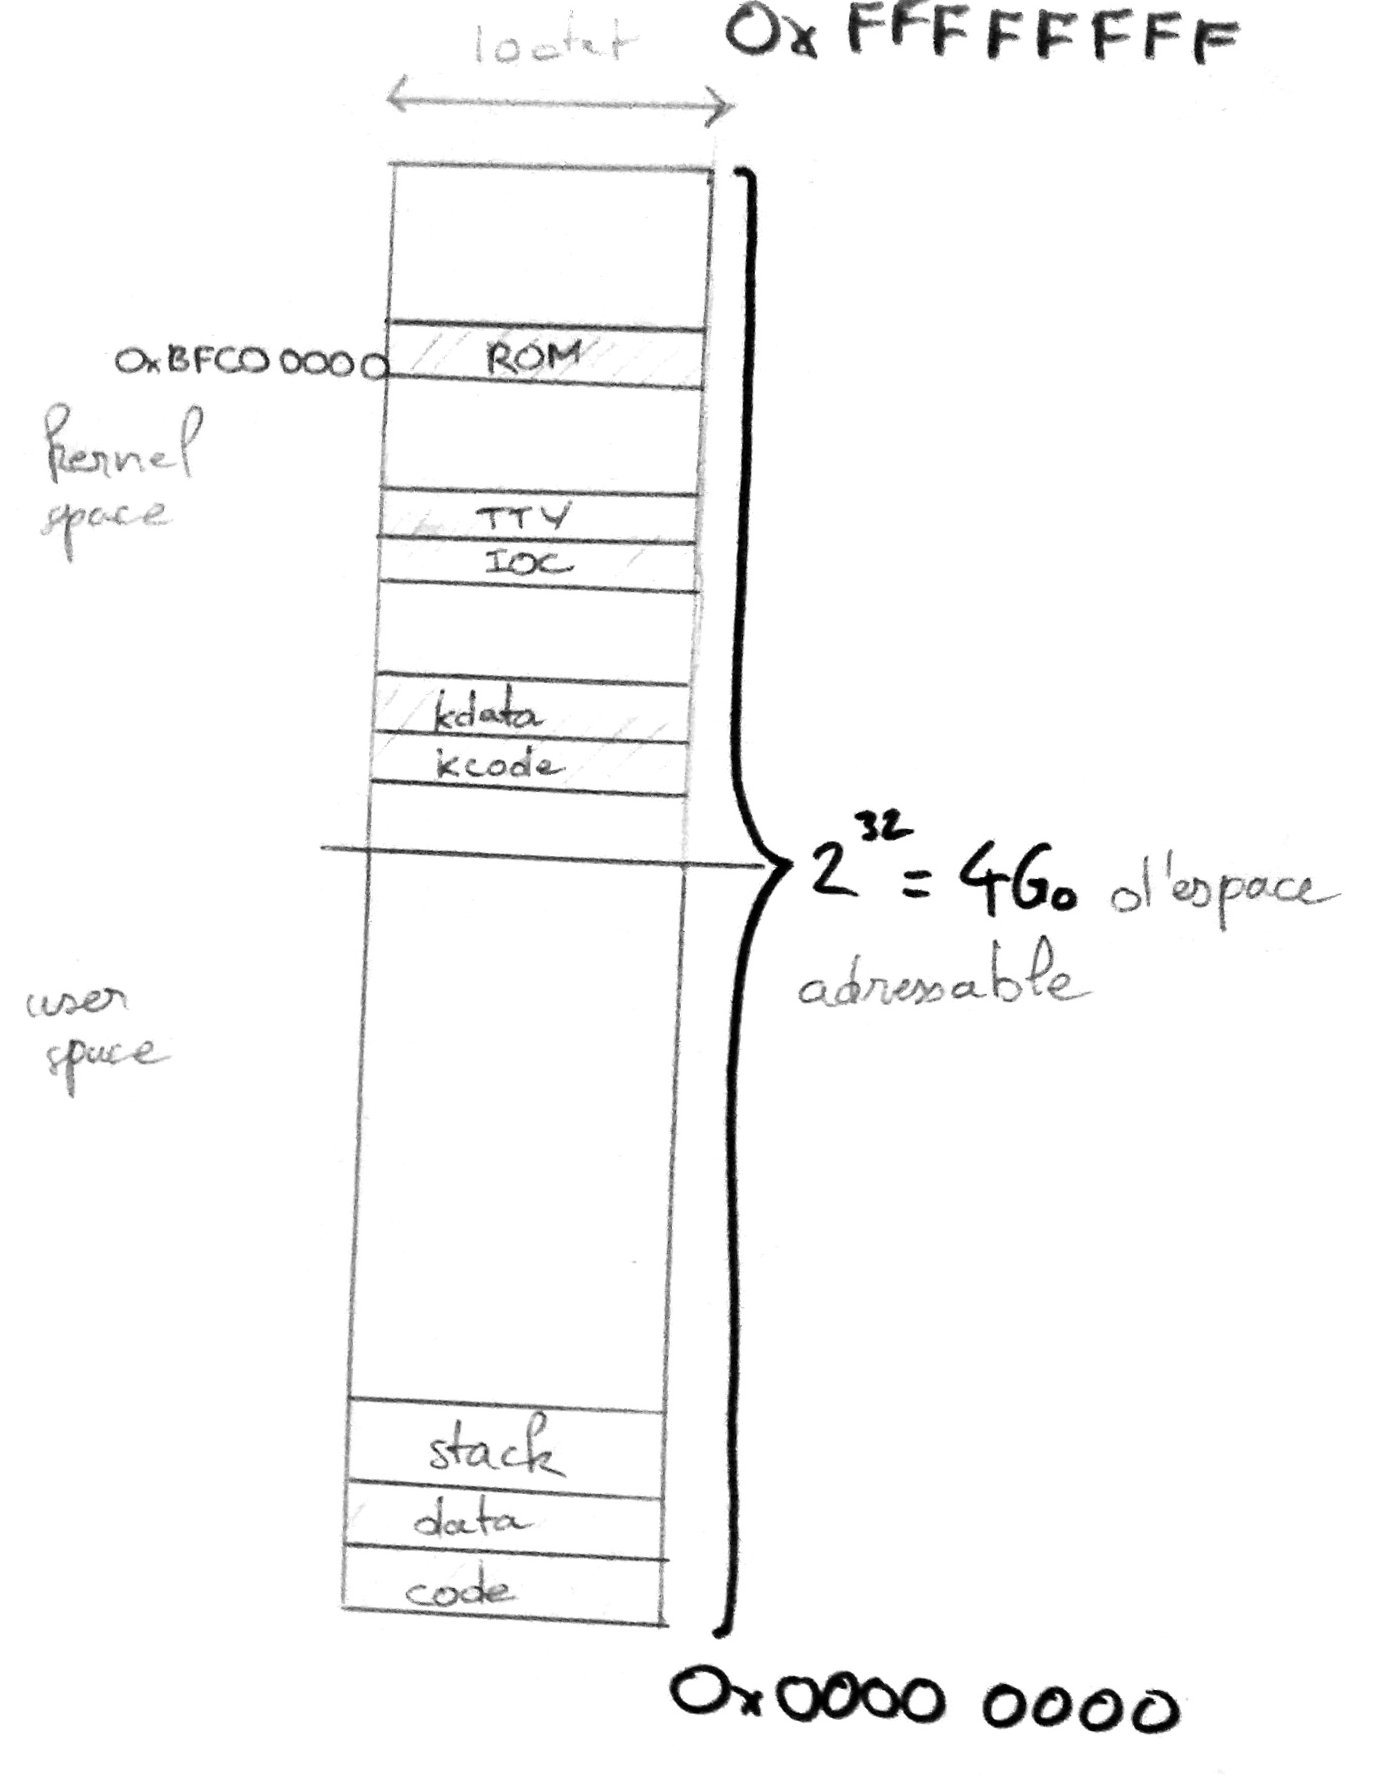
\includegraphics[height=13cm]{cours2/pics/mem.jpg}\\
\end{center}
